\documentclass[a4paper]{article}
\usepackage[utf8]{inputenc}


%=-=-=-=-=-=-=-=-=-=-=-=-=-=-=-=-=-=-=-=-=-=-=-=-=-=-=-=-=-=-=-=-=-=-=-=-=-=-=-=-
% PREAMBLE
%=-=-=-=-=-=-=-=-=-=-=-=-=-=-=-=-=-=-=-=-=-=-=-=-=-=-=-=-=-=-=-=-=-=-=-=-=-=-=-=-

%%%%%%%%%%%%%%%%%%%%%%%%%%%%%%%%%%%%%%%%%%%%%%%%%%%%%%%%%%%%%%%%%%%%%
% Important styling notes
%%
% For now, to include img.jpg in img/path/to/img.jpg, just use:
% path/to/img.jpg - for details see style.tex
%=-=-=-=-=-=-=-=-=-=-=-=-=-=-=-=-=-=-=-=-=-=-=-=-=-=-=-=-=-=-=-=-=-=-=-=-=-=-=-=-
% Packages
%%
%\usepackage{fullpage} % Package to use full page
\usepackage[top=1in,bottom=1in,left=1in,right=0.7in,heightrounded]{geometry}

\usepackage{parskip}                    % Package to tweak paragraph skipping
\usepackage{amsmath}                    % standard
\usepackage{amssymb}                    % standard - Double R symbol etc.
\usepackage{hyperref}
\usepackage{amsthm}                     % standard - theorem, definition, etc.
\usepackage{multicol}                   % multiple columns for numbering
\usepackage{enumitem}                   % standard - enumerate styles
\usepackage[utf8]{inputenc}
\usepackage{scrextend}                  % indentation
\usepackage{graphicx}                   % standard - add figures
\usepackage{float}                      % standard - figure position, use [H] option
\usepackage{pifont}                     % symbols
\usepackage{gensymb}                    % degree symbol \degree
\usepackage{xcolor}                     % bg color
\hypersetup{
    colorlinks,
    linkcolor={black!50!black},
    citecolor={blue!50!black},
    urlcolor={blue!80!black}
}
\usepackage{framed}                     % bg color
\usepackage[T1]{fontenc}                % small caps
\usepackage{sectsty}                    % headings colour
\usepackage{mathtools}                  % Loads amsmath
\usepackage{amsthm,thmtools,xcolor}     % coloured theorem
\usepackage[toc,page]{appendix}         % reference to appendix
%\usepackage{titlesec}                   % change chapter, section, etc. formats
\usepackage{xifthen}                    % if, else
\usepackage{etoolbox}
% format numbering in theorem, lemma, etc. environment
\AtBeginEnvironment{theorem}{\setlist[enumerate, 1]{font=\upshape,  wide=0.5em, before=\leavevmode}}
\AtBeginEnvironment{lemma}{\setlist[enumerate, 1]{font=\upshape,  wide=0.5em, before=\leavevmode}}
\usepackage[letterspace=150]{microtype} % \textls{<letterspaced text>} % 0 <= letterspace <= 1000, 1000 = M space
\usepackage{letltxmacro}                % renew commands?
\usepackage{minted}                     % package to list code
    % otherwise minted goes off the page
    \setmintedinline{breaklines}
\usepackage{subfig}
\usepackage{eso-pic}                    % title page bg pic
\usepackage{varwidth}
\PassOptionsToPackage{svgnames}{xcolor}
\usepackage{fontawesome}                % \faQuestionCircle
\usepackage{marvosym}                   %\Pointinghand
\usepackage{mdframed}                   % easy outline frames
\usepackage[many]{tcolorbox}            % colour box for theorem styles
\usepackage{array,booktabs,calc} % table figs and text
\usepackage{comment}                    % \begin{comment}
\usepackage{fancyhdr}                   % page headings
\usepackage{mdframed}                   % boxes
\usepackage[backend=biber,sorting=none,style=ieee]{biblatex}
\usepackage{caption}
%%% caption options {
%\DeclareCaptionFont{white}{\color{white}}
\DeclareCaptionFormat{listing}{\colorbox{magenta!30!gray}{\parbox{\textwidth}{#1#2#3}}}
\captionsetup[lstlisting]{format=listing,labelfont={bf,small},textfont=small,skip=-1pt}
%%% }
\addbibresource{bibliography.bib}
\usepackage{url}
\usepackage{textcomp}
\usepackage[makeroom]{cancel}            % crossed symbols
\usepackage{algorithm}
\usepackage[noend]{algpseudocode}
\usepackage{tikz}
\usetikzlibrary{arrows.meta,positioning,quotes} % arrows and nodes in tikz
\usepackage{marginnote}
\usepackage{pgfplots}
\usepackage{pstricks-add,pst-slpe}  % for fancy tikz arrows
%\usepackage{titlesec}                   % title style
\usepackage{lmodern}                    % a font
\usepackage{titletoc} % Required for manipulating the table of contents
\usepackage{titlesec} % Allows customization of titles
\usepackage{fouriernc} % Use the New Century Schoolbook font
\usepackage{booktabs} % things in page margins
\usepackage{stmaryrd } % \varoast
\usepackage{listings} % code listings
\usepackage{longtable} % table across multiple pages
\usepackage{styles/nasm/lang}  % include custom language for NASM assembly.
\usepackage{styles/nasm/style} % include custom style for NASM assembly.



%% extra comments that I don't know where they belong:
% list of ding tags: http://willbenton.com/wb-images/pifont.pdf

%=-=-=-=-=-=-=-=-=-=-=-=-=-=-=-=-=-=-=-=-=-=-=-=-=-=-=-=-=-=-=-=-=-=-=-=-=-=-=-=-
% Colours for various things
%%


\definecolor{shadecolor}{rgb}{1.,0.933,0.96} % bg color, r,g,b <= 1
\definecolor{medium_blue}{RGB}{60,125,190}
\definecolor{dark_blue}{RGB}{25,60,85}
\definecolor{dark_red}{RGB}{77,16,16}
\definecolor{LightPink}{rgb}{0.92.,0.8,0.84} % bg color, r,g,b <= 1
\definecolor{LighterPink}{rgb}{1.,0.94,0.97} % bg color, r,g,b <= 1
\definecolor{LightestPink}{rgb}{1.,0.95,0.99} % bg color, r,g,b <= 1
\definecolor{DarkestPink}{rgb}{0.36, 0.0, 0.18}
\definecolor{DarkerPink}{rgb}{0.41, 0.0, 0.21}
\definecolor{DarkPink}{rgb}{0.55, 0.05, 0.37}
\definecolor{lightestestpink}{RGB}{255,248,252}
\definecolor{codegray}{rgb}{0.5,0.5,0.5}
\definecolor{codegrayblue}{rgb}{0.35,0.35,0.47}



%=-=-=-=-=-=-=-=-=-=-=-=-=-=-=-=-=-=-=-=-=-=-=-=-=-=-=-=-=-=-=-=-=-=-=-=-=-=-=-=-
% Define my own theorem styles
%%

% "base" styles
\declaretheoremstyle[
  headfont=\color{DarkPink}\bfseries,
  bodyfont=\itshape,
]{colored}

\declaretheoremstyle[
  headfont=\color{DarkPink}\bfseries,
  bodyfont=\normalfont,
]{colored_upright}

% theorems (corollaries, etc) themselves, inherit from my style above
% Usage:
% \begin{theorem} \end{theorem}, \begin{lemma} \end{lemma}, ...
\declaretheorem[
	numberwithin=section,
 	style=colored,
	name=\textsc{Theorem},
]{theorem}

\tcolorboxenvironment{theorem}{
  boxrule=0pt,
  boxsep=2pt,
  colback={magenta!25!white},
  colframe=DarkPink,
  enhanced jigsaw, 
  borderline west={2pt}{0pt}{DarkPink},
  sharp corners,
  before skip=5pt,
  after skip=5pt,
  breakable,
  right=0mm % for equations
}

\declaretheorem[
	numberwithin=section,
 	style=colored,
	name=\textsc{Corollary},
]{corollary}

\tcolorboxenvironment{corollary}{
  boxrule=0pt,
  boxsep=1pt,
  colback={magenta!10!white},
  colframe=DarkPink,
  enhanced jigsaw, 
  borderline west={2pt}{0pt}{DarkPink},
  sharp corners,
  before skip=5pt,
  after skip=5pt,
  breakable,
  right=0mm % for equations
}

\declaretheorem[
	numberwithin=section,
	style=colored,
	name=\textsc{Lemma},
]{lemma}

\tcolorboxenvironment{lemma}{
  boxrule=0pt,
  boxsep=1pt,
  colback={magenta!10!white},
  colframe=DarkPink,
  enhanced jigsaw, 
  borderline west={2pt}{0pt}{DarkPink},
  sharp corners,
  before skip=5pt,
  after skip=5pt,
  breakable,
  right=0mm % for equations
}

\declaretheorem[
	numberwithin=section,
	style=colored,
	name=\textsc{Definition},
]{definition}

\tcolorboxenvironment{definition}{
  boxrule=0pt,
  boxsep=1pt,
  colback={magenta!25!white},
  colframe=DarkPink,
  enhanced jigsaw, 
  borderline west={2pt}{0pt}{DarkPink},
  sharp corners,
  before skip=5pt,
  after skip=5pt,
  breakable,
  right=0mm % for equations
}

\declaretheorem[
	numberwithin=section,
  	style=colored,
  	name=\textsc{Example},
]{exmp}

\declaretheorem[
	numberwithin=section,
  	style=colored,
  	name=\textsc{Solution},
]{soln}

%%% code listings
\lstdefinestyle{code1}{
    backgroundcolor=\color{lightestestpink},   
    commentstyle=\color{codegrayblue},
    keywordstyle=\color{DarkerPink},
    numberstyle=\tiny\color{codegray},
    stringstyle=\color{black!40!cyan},
    basicstyle=\small\ttfamily,
    breakatwhitespace=false,
    breaklines=true,        
    captionpos=t,             
    keepspaces=true,        
    numbers=left,           
    numbersep=5pt,
    showspaces=false, 
    showstringspaces=false,
    showtabs=false,
    tabsize=4
}

\lstset{style=code1}

%=-=-=-=-=-=-=-=-=-=-=-=-=-=-=-=-=-=-=-=-=-=-=-=-=-=-=-=-=-=-=-=-=-=-=-=-=-=-=-=-
% Headers (size, font, colour)
%%




\makeatletter
\renewcommand{\@seccntformat}[1]{\llap{\textcolor{DarkestPink}{\csname the#1\endcsname}\hspace{1em}}}                    
\renewcommand{\section}{\@startsection{section}{1}{\z@}
{-4ex \@plus -1ex \@minus -.4ex}
{1ex \@plus.2ex }
{\normalfont\large\sffamily\bfseries\textcolor{DarkestPink}}}
\renewcommand{\subsection}{\@startsection {subsection}{2}{\z@}
{-3ex \@plus -0.1ex \@minus -.4ex}
{0.5ex \@plus.2ex }
{\normalfont\sffamily\bfseries\textcolor{DarkestPink}}}
\renewcommand{\subsubsection}{\@startsection {subsubsection}{3}{\z@}
{-2ex \@plus -0.1ex \@minus -.2ex}
{.2ex \@plus.2ex }
{\normalfont\small\sffamily\bfseries\textcolor{DarkestPink}}}                        


%=-=-=-=-=-=-=-=-=-=-=-=-=-=-=-=-=-=-=-=-=-=-=-=-=-=-=-=-=-=-=-=-=-=-=-=-=-=-=-=-
% Numberings, counters and spacings
%%
\numberwithin{equation}{section} % section number in eq/s
\setlength{\jot}{7pt} % spacing in split, gathered env/s



%% Custom examples
%% Output - Example 1,2,...
\newcounter{example}
\newenvironment{example}[1][]{\refstepcounter{example}\par\medskip
   \textbf{Example~\theexample. #1} \rmfamily}{\medskip}
%%%%%%%%%%%% End of unused %%%%%%%%%%%%



%=-=-=-=-=-=-=-=-=-=-=-=-=-=-=-=-=-=-=-=-=-=-=-=-=-=-=-=-=-=-=-=-=-=-=-=-=-=-=-=-
% Paths
%%
\graphicspath{ {./img/} } % figures' path - can look up files directly from there


%=-=-=-=-=-=-=-=-=-=-=-=-=-=-=-=-=-=-=-=-=-=-=-=-=-=-=-=-=-=-=-=-=-=-=-=-=-=-=-=-
% User defined macros (math mode)
%%


% Curly braces under text. Usage: \myunderbrace{upper}{lower}
\newcommand{\myunderbrace}[2]{\mathrlap{\underbrace{\phantom{#1}}_{#2}} #1}
\newcommand{\setR}{\mathbb{R}} % \ouble R
\newcommand{\setRn}{\mathbb{R}^n} %  double R^n
\newcommand{\setN}{\mathbb{N}} % double N
\newcommand{\setZ}{\mathbb{Z}} % double Z
\let\oldemptyset\emptyset
\let\emptyset\varnothing % nice - looking empty set symbol
\newcommand{\fancyN}{\mathcal{N}} % null space
\newcommand{\fancyR}{\mathcal{R}} % range

\newcommand{\bx}{\textbf{x}}
\newcommand{\by}{\textbf{y}}
\newcommand{\bb}{\textbf{b}}
\newcommand{\bA}{\textbf{A}}
\newcommand{\bB}{\textbf{B}}
\newcommand{\bI}{\textbf{I}}
% double bars as in norm
\newcommand{\norm}[1] {\lVert #1 \rVert} 
\newcommand{\trans}[1]{#1^{\top}}

\newcommand{\mean}[1]{\bar{#1}}
\newcommand{\var}{\sigma^2}

\newcommand{\partdevx}[1]{\frac{\partial #1}{\partial x}}
\newcommand{\partdevxx}[1]{\frac{\partial #1}{\partial x}}
\newcommand{\partdevxn}[1]{\frac{\partial^n #1}{\partial x^n}}
\newcommand{\partdevy}[1]{\frac{\partial #1}{\partial x}}
\newcommand{\partdevyy}[1]{\frac{\partial #1}{\partial y}}
\newcommand{\partdevyn}[1]{\frac{\partial^n #1}{\partial y^n}}

% text above = symbol
\newcommand{\overeq}[1]{\ensuremath{\stackrel{#1}=}} 
\newcommand{\greatersmaller}{%
  \mathrel{\ooalign{\raisebox{.6ex}{$>$}\cr\raisebox{-.6ex}{$<$}}}
} % greater and smaller symbols on top of each other, same line

%=-=-=-=-=-=-=-=-=-=-=-=-=-=-=-=-=-=-=-=-=-=-=-=-=-=-=-=-=-=-=-=-=-=-=-=-=-=-=-=-
% User defined macros (non math)

\newcommand{\qedblack}{$\hfill\blacksquare$} % black square end of line
\newcommand{\qedwhite}{\hfill \ensuremath{\Box}} % white square end of line
\newcommand{\hquad}{\hskip0.5em\relax}% half quad space
%\newcommand{\TODO}{\textcolor{red}{\bf TODO!}\;}

\newcommand{\TODO}[1][]{%
    \ifthenelse{\equal{#1}{}}{\textcolor{red}{\bf TODO!}\;}{\textcolor{red}{\textbf {TODO:} #1}\; }%
}
\newcommand{\B}[1]{\textbf{\textup{#1}}} % bold and upright
\renewcommand{\labelitemi}{\scriptsize$\textcolor{DarkPink}{\blacksquare}$} % itemize - squares instead of bullets
\newcommand{\emphasis}[1]{\textls{#1}}

\LetLtxMacro{\originaleqref}{\eqref}
\renewcommand{\eqref}{Eq.~\originaleqref}
\renewcommand*{\eqref}[1]{Eq.~\originaleqref{#1}}





% background images
%%%%%%%
\newcommand\BackgroundPic{%
\put(0,0){%
\parbox[b][\paperheight]{\paperwidth}{%
\vfill
%\centering

\includegraphics[width=0.125\paperwidth,height=\paperheight,%
]{img/background_02.png}% use ,keepaspectratio
\vfill
}}}
%%%%%%%
% end of background image
%%%%%%%%%%%%%% my own frame
\newmdenv[topline=false,bottomline=false]{leftrightbox}
%%%%%%%%%%%%% end
%%%%%%%%%%%%% my own comment
\newcommand{\mycomment}[1]{\begin{leftrightbox}\Pointinghand~\textbf{Comment:}~#1 \end{leftrightbox}}
%%%%%%%%%%%%% end
% my custom note https://tex.stackexchange.com/questions/301993/create-custom-note-environment-with-tcolorbox
\newmdenv[
    topline=false,
    bottomline=false,
    rightline=false,
    innerrightmargin=0pt
]{siderule}
\newenvironment{mynote}%
    {\begin{siderule}\textbf{\Pointinghand~Note:}}
    {\end{siderule}}
%%%%%%%%%%%%% my own box
\newcommand{\boxone}[1]{\begin{tcolorbox}[colback = LighterPink,colframe=LightPink]
#1
\end{tcolorbox}}
%%%%%%%%%%%%% end

\let\oldemptyset\emptyset
\let\emptyset\varnothing
%algorithmic
\algdef{SE}[DOWHILE]{Do}{doWhile}{\algorithmicdo}[1]{\algorithmicwhile\ #1}%






\begin{document}
%=-=-=-=-=-=-=-=-=-=-=-=-=-=-=-=-=-=-=-=-=-=-=-=-=-=-=-=-=-=-=-=-=-=-=-=-=-=-=-=-
% GLOBAL STYLES (DOCUMENT SCOPE)
%=-=-=-=-=-=-=-=-=-=-=-=-=-=-=-=-=-=-=-=-=-=-=-=-=-=-=-=-=-=-=-=-=-=-=-=-=-=-=-=-
% caption: Figure 1 -> <bold> Fig. 1 </bold>
\captionsetup[figure]{labelfont={bf},labelformat={default},labelsep=period,name={Fig.}}


%=-=-=-=-=-=-=-=-=-=-=-=-=-=-=-=-=-=-=-=-=-=-=-=-=-=-=-=-=-=-=-=-=-=-=-=-=-=-=-=-
% TITLE PAGE
%=-=-=-=-=-=-=-=-=-=-=-=-=-=-=-=-=-=-=-=-=-=-=-=-=-=-=-=-=-=-=-=-=-=-=-=-=-=-=-=-
%%%%%%%%%%%%%%%%%%%%%%%%%%%%%%%%%%%%%%%%%
% Formal Book Title Page
% LaTeX Template
% Version 2.0 (23/7/17)
%
% This template was downloaded from:
% http://www.LaTeXTemplates.com
%
% Original author:
% Peter Wilson (herries.press@earthlink.net) with modifications by:
% Vel (vel@latextemplates.com)
%
% License:
% CC BY-NC-SA 3.0 (http://creativecommons.org/licenses/by-nc-sa/3.0/)
% 
% This template can be used in one of two ways:
%
% 1) Content can be added at the end of this file just before the \end{document}
% to use this title page as the starting point for your document.
%
% 2) Alternatively, if you already have a document which you wish to add this
% title page to, copy everything between the \begin{document} and
% \end{document} and paste it where you would like the title page in your
% document. You will then need to insert the packages and document 
% configurations into your document carefully making sure you are not loading
% the same package twice and that there are no clashes.
%
%%%%%%%%%%%%%%%%%%%%%%%%%%%%%%%%%%%%%%%%%

%----------------------------------------------------------------------------------------
%	PACKAGES AND OTHER DOCUMENT CONFIGURATIONS
%----------------------------------------------------------------------------------------



%----------------------------------------------------------------------------------------
%	TITLE PAGE
%----------------------------------------------------------------------------------------



\begin{titlepage} % Suppresses headers and footers on the title page

	\centering % Centre everything on the title page
	
	\scshape % Use small caps for all text on the title page
	
	\vspace*{\baselineskip} % White space at the top of the page
	
	%------------------------------------------------
	%	Title
	%------------------------------------------------
	
	\rule{\textwidth}{1.6pt}\vspace*{-\baselineskip}\vspace*{2pt} % Thick horizontal rule
	\rule{\textwidth}{0.4pt} % Thin horizontal rule
	
	\vspace{0.75\baselineskip} % Whitespace above the title
	
	{\LARGE COMPUTER VISION NOTES\\ \Large OBJECT LOCALISATION AND TRACKING\\} % Title
	
	\vspace{0.75\baselineskip} % Whitespace below the title
	
	\rule{\textwidth}{0.4pt}\vspace*{-\baselineskip}\vspace{3.2pt} % Thin horizontal rule
	\rule{\textwidth}{1.6pt} % Thick horizontal rule
	
	\vspace{2\baselineskip} % Whitespace after the title block
	
	%------------------------------------------------
	%	Subtitle
	%------------------------------------------------
	My personal notes on
	
	\vspace*{3\baselineskip} % Whitespace under the subtitle
	
	Object Localisation Techniques; Colour Matching, Mean Shift Tracking, Optical Flow, Lukas Kanade 
	
	\vspace*{3\baselineskip} % Whitespace under the subtitle
	
	%------------------------------------------------
	%	Editor(s)
	%------------------------------------------------
	
	By
	
	\vspace{0.5\baselineskip} % Whitespace before the editors
	
	{\normalfont \Large \mintinline{latex}{0xLeo} (\url{github.com/0xleo}) \\} % Editor list
	
	\vspace{0.5\baselineskip} % Whitespace below the editor list
	
	%\textit{The University of California \\ Berkeley} % Editor affiliation
	
	\vfill % Whitespace between editor names and publisher logo
	
	%------------------------------------------------
	%	Publisher
	%------------------------------------------------
	
	
	\vspace{0.3\baselineskip} % Whitespace under the publisher logo
	
	\today % Date
	
	{DRAFT X.YY} % Draft version
	{\\Missing: \ldots}

\end{titlepage}

%----------------------------------------------------------------------------------------

%\maketitle



%=-=-=-=-=-=-=-=-=-=-=-=-=-=-=-=-=-=-=-=-=-=-=-=-=-=-=-=-=-=-=-=-=-=-=-=-=-=-=-=-
% MAIN DOCUMENT
%=-=-=-=-=-=-=-=-=-=-=-=-=-=-=-=-=-=-=-=-=-=-=-=-=-=-=-=-=-=-=-=-=-=-=-=-=-=-=-=-
\newpage
\tableofcontents
\newpage



%------------------------------ New section ------------------------------%
\section{Viola Jones detection}


\subsection{Problem statement and idea}
Detecting faces is complicates since they have so many features, such as forehead, eyes, lips etc. Faces can also be in any size and position through the image, they can be non-uniformly illuminated, have multiple expressions or be occluded. Viola Jones takes advantage of the fact that every face has certain characteristics, that such the nose usually brighter is darker than the surrounding cheek area, the eye pupil is darker than the sclera, the nose, lip and eye position relative to each other etc. Viola Jones works in real time by combining the following methods:
\begin{enumerate}
    \item Integral image. This speeds up the feature computation time.
    \item Haar features. These are simple rectangular masks that resemble with Haar wavelets.
    \item Boosting for feature selection (``AdaBoosting''). Iteratively classifies good and bad features.
    \item Cascade of weak feature classifiers to quickly reject windows without faces (Attentional cascade).
\end{enumerate}
Viola Jones scans a window that searches features over the image, incrementing pixel by pixel. The window size remains constant -- the authors of VJ suggest $24\times 24$ window the image is considered at various scales -- the authors suggest a scaling factor of $1.25$.  All the scalings along with the original image are called \emphasis{image pyramid}. Each level in the pyramid is obtain by downsampling the previous. For example, downsampling of $1.25$ implies that every 5 pixels we save 4 and reject the 5th.
% ref https://www.mpi-inf.mpg.de/fileadmin/inf/d2/HLCV/cv-ss13-0605-sliding-window.pdf
\begin{figure}[H]
    \centering
    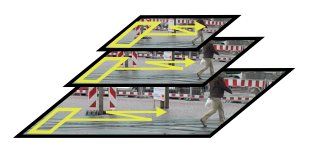
\includegraphics[height=2.5cm]{img/window_slide_loc_scale.PNG}
    \caption{Same window scans different image scales.}
\end{figure}
The window contains a different feature detector each time, e.g. one that might detect an eye or one that might detect a nose. \textit{Haar features} determine what we want to compute each time, e.g. an eye, a forehead etc. One might think that the larger the window, the larger the number of operations done to compute the feature inside it. We will see that the number of computations is always constant thanks to the idea of \textit{integral image}, whose computation is the first step of the algorithm. Why integral image is useful will be shown later, next section explains  how it's computed. To summarise, the whole algorithm is explained by the following high-level pseudocode.
% src https://sites.google.com/site/5kk73gpu2012/assignment/viola-jones-face-detection
\begin{verbatim}
for number of scales in image pyramid do
    downsample image by one scale
    compute integral image for current scale
    for each shift step of the sliding detection window do
        for each stage in the cascade classifier do
            for each filter in the stage do
                filter the detection window
            end
            accumulate filter outputs within this stage
            if accumulation fails to pass per-stage threshold do
                break the for loop and reject this window as a face
            end
        end
        if this detection window passes all per-stage thresholds do
            accept this window as a face
        else
            reject this window as a face
        end
    end
end
\end{verbatim}


\subsection{Integral image}
Given the source image $ii(x,y)$ where we want to detect faces, a new, \emphasis{integral  image}  $i(x,y)$ is  created such that each  new pixel is the sum of the pixels above and to the left of it, including the original pixel itself:
\begin{equation}
    ii(x,y) = \sum\limits_{x\prime \leq x,\ y\prime \leq y} i(x\prime, y\prime)
\end{equation}
\begin{multicols}{2}
\begin{figure}[H]
    % ref: comphile viola jones
    \centering
    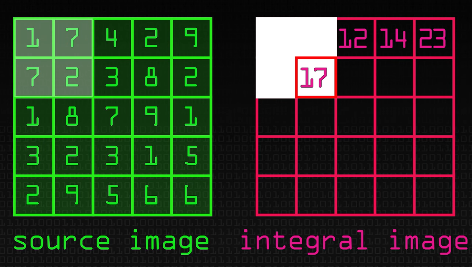
\includegraphics[height=2.5cm]{img/int_image_one_pixel.png}
    \caption{Computing a single pixel of the integral image.}
\end{figure}
\columnbreak
\begin{figure}[H]
    \centering
    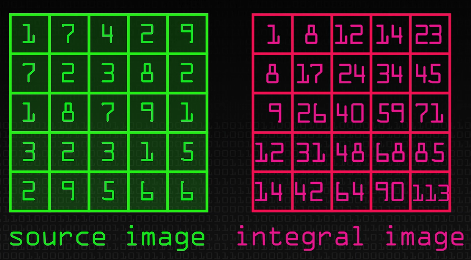
\includegraphics[height=2.5cm]{img/int_image_whole.png}
    \caption{The whole integral image computed.}
\end{figure}
\end{multicols}
This technique allows constant time ($\mathcal{O}(1)$) calculation of the sum of all pixels within a rectangle. 
\begin{figure}[H]
    % https://pdfs.semanticscholar.org/40b1/0e330a5511a6a45f42c8b86da222504c717f.pdf
    \centering
    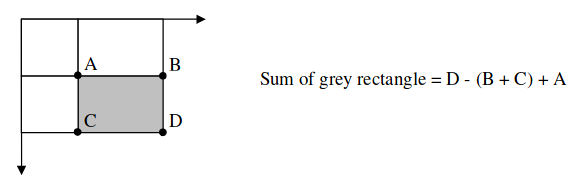
\includegraphics[height=3.5cm]{img/int_image_rectangle.png}
    \caption{Rectangle sum calculation. The rectangles from the origin to A, B, C, D are pre-computed by the integral image. A is counted in both B and C so in the end we subtract it.}
    \label{fig:my_label}
\end{figure}
Sums of pixels are computed in order to find the Haar features described in the next sections. Since we have tons of Haar features, pre-computing the integral image is necessary.



\subsection{Haar features}
\marginnote{Haar features are supposed to be similar to simple face features found in the nose, eyes, etc.}But what exactly are the Haar features and how do they look like? They are simple rectangular masks and each one is supposed to roughly resemble with a certain face feature, e.g. the left end of the lip. They contain certain combinations of zeros and ones. Ones should match bright areas of the feature and zeros dark. Haar features are always located in the sliding window and they are used similarly to convolution kernels.
\begin{figure}[H]
    \centering
    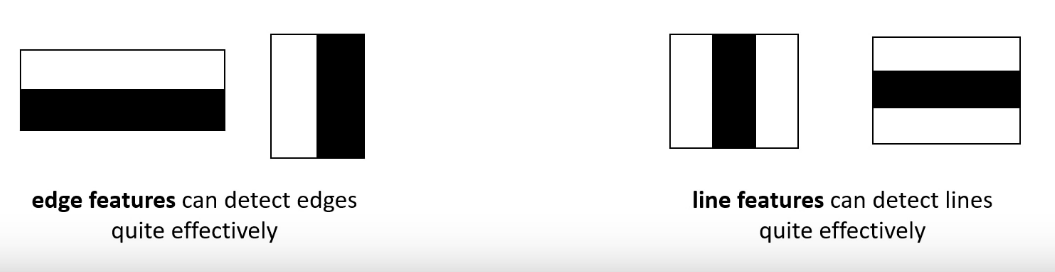
\includegraphics[height=2.5cm]{img/haar_simple_feat.png}
    \caption{Some Haar features for line and edge detection.}
\end{figure}
For example, the edge feature in the above figure could roughly match an eyebrow and the vertical line feature could match the now bridge, as shown below. Of course, line features can also be diagonal to detect rotated faces.
\begin{figure}[H]
    \centering
    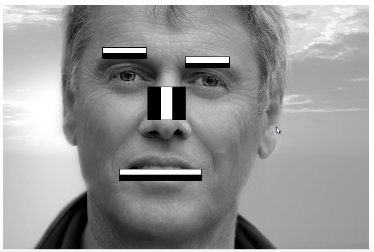
\includegraphics[height=3.75cm]{img/haar_feat_face.png}
    \caption{Some Haar features that match face features.}
\end{figure}
To measure the quality of a feature, i.e. its similarity to the overlapping Haar cascade, we simply subtract the pixels under the black ones from those under the whites and divide the result by the size of the Haar feature. The higher the result $\Delta$, the more likely a feature to belong to a face. This method is also called ``difference of adjacent boxes''. Below, $n$ of the number of pixels of the Haar feature.
\begin{equation}
    \Delta = \textup{dark} - \textup{white} = \frac{1}{n} \sum \limits_{\substack{(x,y)\\ \textup{under}\;\textup{white}}}i(x,y)
    - \frac{1}{n} \sum \limits_{\substack{(x,y)\\ \textup{under}\;\textup{black}}}i(x,y)
\end{equation}
The two figures below explain the $\Delta$ calculations. For the feature in Fig. \ref{fig:downsampled_eyebrow}, we have \footnote{Images are represented as 8-bit integers so a negative result would be clipped to 0 and one that cannot be represented by 8 bits to $255$.}
\[
\Delta = \frac{1}{16} (209 + 214 + 207 + 199 + 183 + 196 + 200+ 212 - 181 - 77 - 105 - 67 - 68-101 - 183 - 196) = 40.125
\]
The closer the value of $\Delta$ to $255$, the better the feature. A region of random pixels would have $\Delta \approx 0$. This calculation seems quite fast but it needs to be repeated for a huge number of times. When the Haar rectangle is large, it adds up a lot of computation time.
\begin{figure}[H]
    \centering
    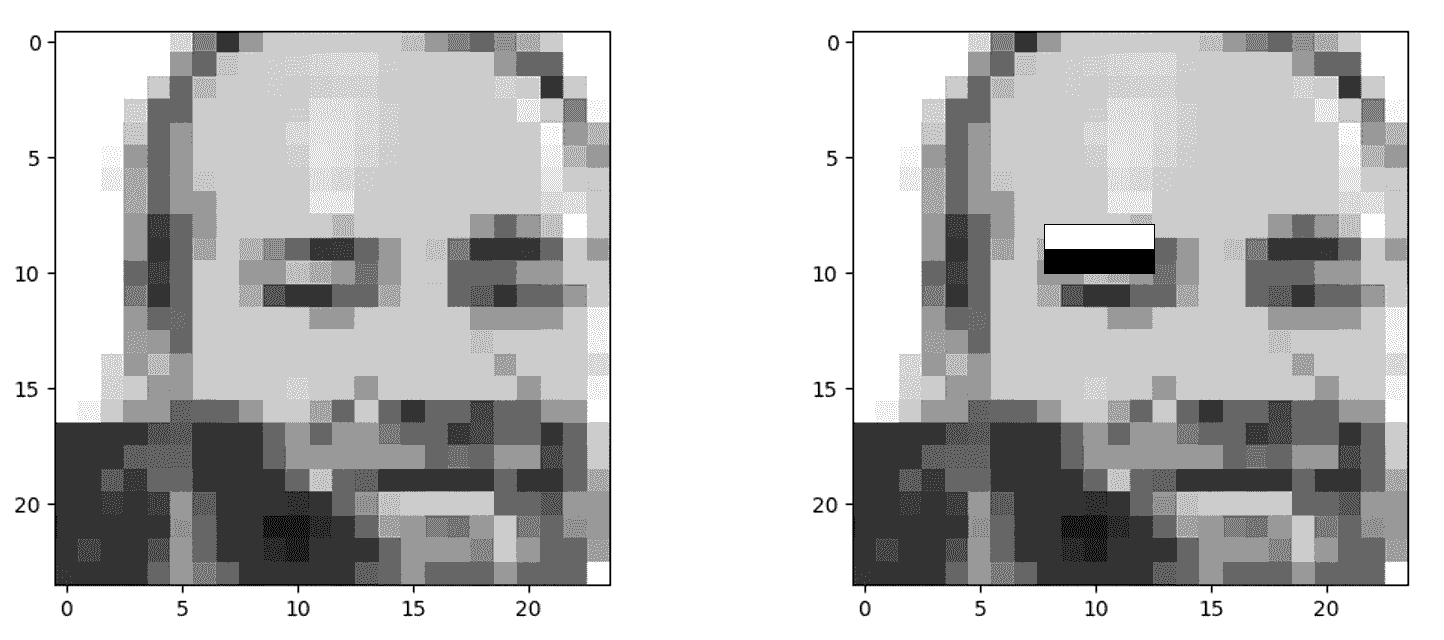
\includegraphics[height=3cm]{img/downsampled_human_face.png}
    \caption{The sliding $24\times 24$ window captures a downsampled face. A line feature is overlaid the eyebrow.}
\end{figure}
\begin{figure}[H]
    \centering
    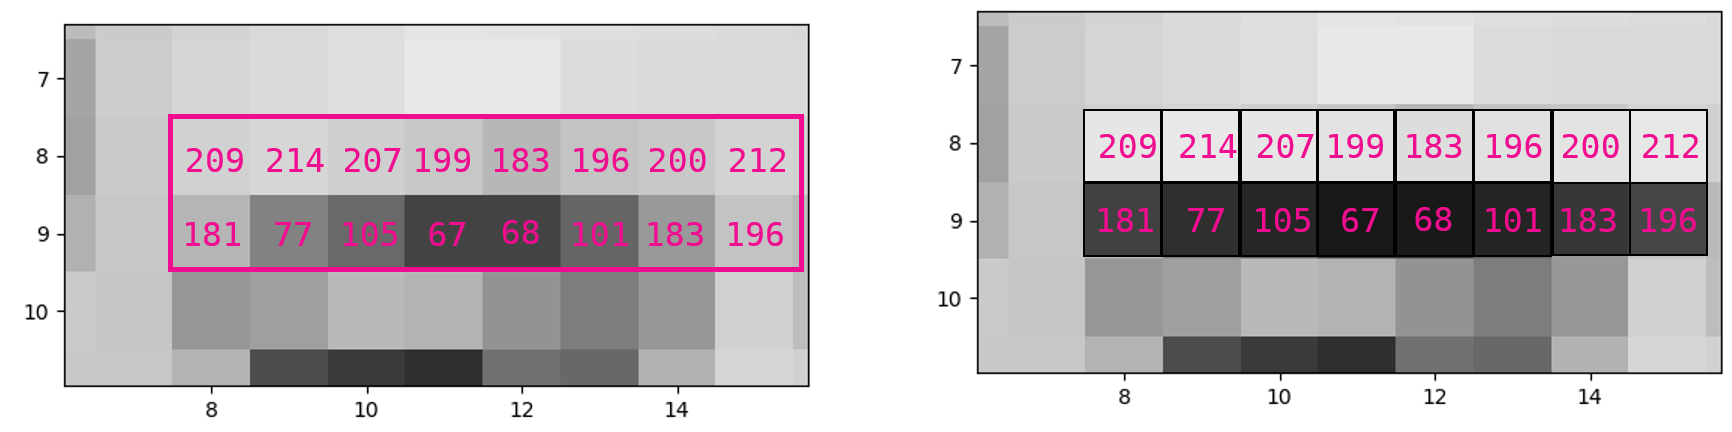
\includegraphics[height=3.0cm]{img/downsampled_human_eyebrow.png}
    \caption{A closer look at the intensity values of the eyebrow. Pixels  under the black region will be subtracted and those under the white region will be added.}
    \label{fig:downsampled_eyebrow}
\end{figure}
\marginnote{Integral image speeds up the Haar feature computation.}This is where integral image discussed in the previous section comes in handy. Instead of calculating the sum naively, for Fig. \ref{fig:downsampled_eyebrow} we would find the sum inside the white and black rectangles using the integral image. Therefore each black or white sub-rectangle only requires 4 additions. 
\begin{figure}[H]
    %ref https://www12.cs.fau.de/edu/map/ss15/talks/vj_cuda.pdf
    \centering
    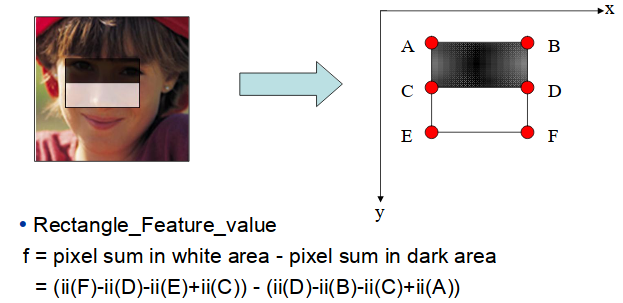
\includegraphics[height=4.75cm]{img/haar_line_int_image.png}
    \caption{Computing an example Haar feature using the integral image $ii$.}
    \label{fig:my_label}
\end{figure}
By comparing each $\Delta$ value to a threshold, e.g. $30$ we can tell if the region under the window is likely to be a face, although this procedure will give lots of \textit{false positives}. If the result is less than $30$, then that feature in that window position will not be considered. If it's greater, more Haar classifiers will be applied. That's called a \textit{weak classifier} and the algorithm combines multiple of them. ``Weak essentially means better than random classifier, so in this case as long as the classifier outputs a value roughly greater than zero, then the window is likely to contain a face:
\begin{equation}
    y(\Delta_{\boldsymbol{\theta}})= \left\{
\begin{array}{ll}
      1, & \Delta_{\boldsymbol{\theta}} > T\\
      0, & \textup{else} \\
\end{array} 
\right. 
\end{equation}
, where $\boldsymbol{\theta}$ refers to a set of parameters such as the number of rectangles, their positions, etc. The problem with using Haar features inside the window is that for a $24\times 24$ window there are about $160,000$ of them, so computing them all is inefficient. The algorithm needs to select and combine in advance some good Haar features. This is done by a machine learning algorithm called ``AdaBoost''.





%The formula is demonstrated in the following figure.\\
%\TODO[example from yt]\\
%\TODO[also very good:]
%\url{http://www.botmag.com/images/drupal/ViolaJones_Simplified_byEricGregori.pdf}\\
%This is where integral image comes in handy. \TODO\\
%\TODO[how to choose features?]\\
%\url{https://stackoverflow.com/questions/27322848/defining-an-initial-set-of-haar-like-features}\\
%\url{https://docs.opencv.org/3.4/db/d28/tutorial_cascade_classifier.html}

\subsection{Adaboost training}
The solution to the fact that the sliding window contains over $160,000$ features is to select a few of them -- the most reliable ones that can tell whether the sub-image contains a face. This is done by AdaBoost (adaptive boost), which is a topic on its own, so it won't be discussed in too much detail but this section includes the overview.

For a certain position of the sliding window and given its features $f_1,f_2,\ldots$ such as position of black boxes, coordinates, threshold etc, the idea is that we have a set of data and outputs $(\bx_1, y_1), \ldots, (\bx_m, y_m),\ \bx \in \setR^d,\ y \in \{-1,1\}$ ($-1$: is not face, $1$: is face) and we want to train perceptrons to correctly classify the output points, i.e. we want to linearly classify them. The goal is to find the features that best separate the positive and negative classes. 
% mpore about features 
\begin{figure}[H]
    \centering
    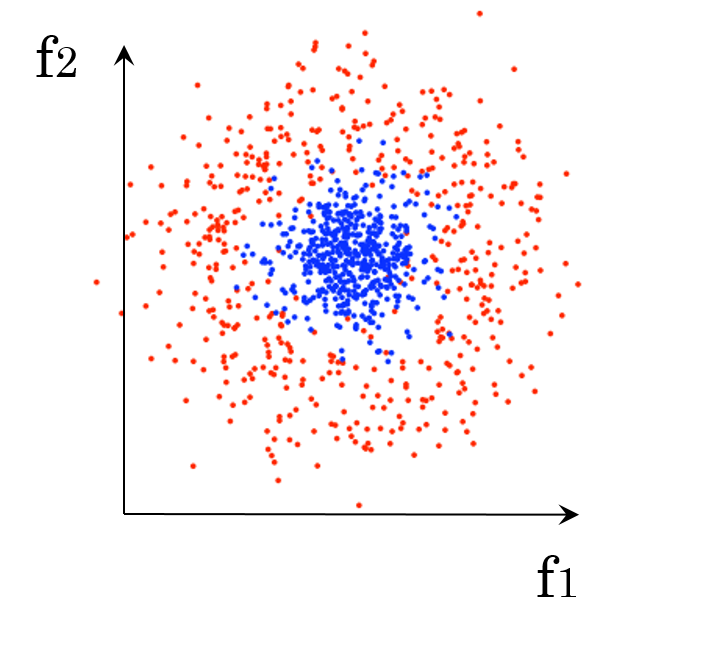
\includegraphics[height=4cm]{img/feature_pts.png}
    \caption{Various data points $\left((x_{i1},x_{i2}),y_i\right)$} in the 2D feature space $f_1,f_2$. Each class is represented by a colour.
\end{figure}
% ref http://www.robots.ox.ac.uk/~az/lectures/cv/adaboost_matas.pdf
Adaboost aims to separate the data in two classes, minimising some error function. It constructs a ``strong'' linear classifier as a combination of $T$ simple ``weak'' simple linear classifiers $h^{(1)}(x), \ldots, h^{(T)}(x)$:
\begin{equation}
    f(x) = \sum\limits_{t=1}^{T}{\alpha^{(t)}h^{(t)}(x)}
\end{equation}
, where:
\begin{itemize}
    \item $h_t(x)$ is a ``weak'' or base classifier -- can be a perceptron, or decision tree etc, as long as it can perform linear binary classification.    
    \item $H(x) = \textup{sgn}\left(f(x)\right)$ is the final, strong, classifier.
    \item $\alpha^{(t)}$ is a coefficient we set at each iteration depending on how good the base classifier $h^{(t)}$ is.
\end{itemize}
\marginnote{AdaBoost essentially applies a series of linear classifiers, increasing the weights of the errors and decreasing the correct ones each iteration.}The algorithm maintains a weight distribution $\bw^{(t)} = (w^{(t)}_1,\ldots,w^{(t)}_m)$ over the data points \footnote{Weights $\bw^{(t)}$ and $\alpha_1,\ldots,\alpha_m$ are different.}. The weights $w^{(t)}$ are initialised uniformly, and are updated in each iteration, keeping their sum constant, e.g. normalised. The goal of the base learner is to minimise the \textit{weighted (base) error}
\begin{equation}
    \epsilon^{(t)} = \sum_{i=0}^{m}{w^{(t)}_i}I\left\{h^{(t)}(\bx_i)\neq y_i \right\}
\end{equation}
, where $I(true) = 1, \ I(false) = 0$ so $\epsilon^{(t)}$ can be considered as the sum of the weights of the wrong examples \footnote{There are better error functions than this sum but we don't discuss them here for simplicity.}, i.e. $\sum_{h^{(t)}(\bx_i)\neq y_i}w^{(t)}_i$. 

Having found the total error, the weak classifier weight $\alpha^{(t)}$ is set as
\begin{equation}
    \alpha^{(t)} = \frac{1}{2}\ln{\frac{1-\epsilon^{(t)}}{\epsilon^{(t)}}}
\end{equation}
So the larger the error $\epsilon^{(t)}$, the smaller the weight $\alpha^{(t)}$. The final pseudocode is shown below. We denote the training set as $\mathcal{D}_m = \left\{(\bx_1,y_1),\ldots,(\bx_m,y_m) \right\}$

% ref https://users.lal.in2p3.fr/kegl/teaching/stages/notes/tutorial, http://www.robots.ox.ac.uk/~az/lectures/cv/adaboost_matas.pdf
\begin{algorithm}[H]
\caption{AdaBoost algorithm outline.}
\label{alg:hist_backproj}
\begin{algorithmic}[1]
\Procedure{AdaBoost} {$\mathcal{D}_m$, Base(.,.), $T$} 
\State $w^{(1)} \leftarrow (1/m, \ldots, 1/m)$ \Comment{initial weights}
\For{$t \leftarrow 1,\ldots,T$} 
\State $h^{(t)} \leftarrow Base(\mathcal{D}_m,\bw^{(t)})$ \Comment{apply base classifier; e.g. a simple perceptron}
\State $\epsilon^{(t)} \leftarrow \sum_{i=0}^{m}{w^{(t)}_i}I\left\{h^{(t)}(\bx_i)\neq y_i \right\}$ \Comment{weighted (total) error of base classifier $t$}
\State $\alpha^{(t)} \leftarrow \frac{1}{2}\ln{\frac{1-\epsilon^{(t)}}{\epsilon^{(t)}}}$
\For{$i \leftarrow 1,\ldots,m$} \Comment{re-weight each training point}
\If {$h^{(t)}(t)\neq y_i$} \Comment{error}
\State $w^{(t+1)}_i \leftarrow \frac{w_i^{(t)}}{2\epsilon^{(t)}}$ \Comment{increase the weight}
\Else \Comment{correct classification}
\State $w^{(t+1)}_i \leftarrow \frac{w_i^{(t)}}{2\left(1-\epsilon^{(t)}\right)}$ \Comment{decrease the weight}
\EndIf
\EndFor
\EndFor
\State \textbf{return} $\textup{sgn}\left(f(\bx)\right)=\textup{sgn}\left(\sum\limits^{T}_{t=1}\alpha^{(t)}h^{(t)}(\bx)\right)$ \Comment{weighted ``vote'' of best (a.k.a. base) classifiers}
\EndProcedure
\end{algorithmic}
\end{algorithm}
It's important to remember the weights are normalised for each iteration of the algorithm, i.e.
\begin{equation}
    \sum\limits_{i=1}^{m}w_i^{t}=1
\end{equation}
\begin{figure}[H]
    \centering
    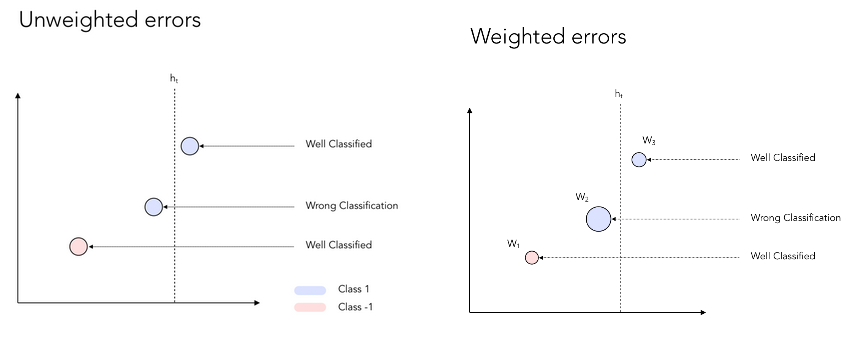
\includegraphics[height=4.5cm]{img/ada_wrong_examples_weights.png}
    \caption{Weights of wrong examples are increased and weights of correct ones are decreased.}
\end{figure}
The figure below shows how the weights are updated at every iteration.
\begin{figure}[H]
    % ref https://www12.cs.fau.de/edu/map/ss15/talks/vj_cuda.pdf
    \centering
    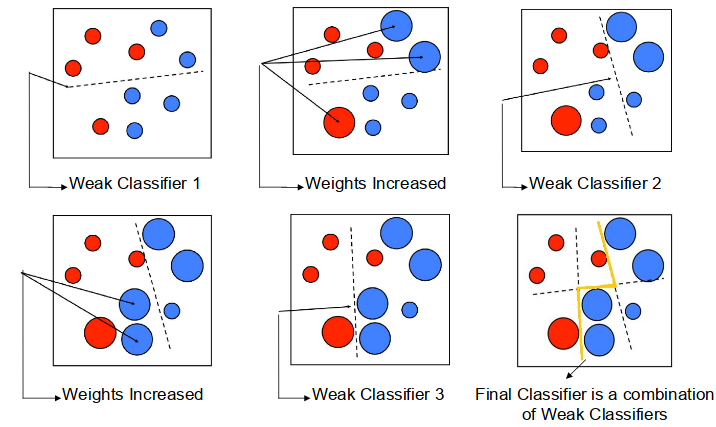
\includegraphics[height=6cm]{img/ada_adjusting_weights.png}
    \caption{At every iteration $t$ the weights of false classifications are increased and the correct ones are decreased. Then the base classifier $h^{(t)}$ is applied again.}
\end{figure}



\subsection{Classifier cascade}
So far, we applied various Haar masks of different sizes, formations, and locations, etc (there are the features $\bx^{(i)}\in \setR^d$, where $d$ the total number of sizes, formations, and locations etc), compared the summation result of masking calculated using the integral image to a threshold, and depending on the comparison result we classified the output $y^{(i)} \in \{-1,1\}$ as ``is in face'' ($1$) or ``is not in face'' ($-1$). Then we separate all positive and negative results in two groups using a strong classifier calculated by AdaBoost. We had been dealing with only a fixed image size (no scales).  

% ref https://medium.com/datadriveninvestor/understanding-and-implementing-viola-jones-part-two-97ae164ee60f
\marginnote{Each part of the cascade operates on a different input scale.}
For a large image, and considering the image will have to be scaled and rescaled to account for differently sized faces, this amounts to using Viola-Jones a large number of times. If the system needs to detect faces in real-time, the computation needs to be fast. It is for this purpose that Viola and Jones introduced the \emphasis{attentional cascade}.

% ref https://medium.com/datadriveninvestor/understanding-and-implementing-viola-jones-part-two-97ae164ee60f
The attentional cascade uses a series of strong classifiers (see previous section), each progressively having more features, to classify an image. An image is only put through by the $n$th classifier (larger image size) if the $n-1$th classifier (smaller size) classifies it as a positive example. If at any point a classifier does not think the image is a positive example, the cascade stops and the region is rejected as a face. The reason behind it is that in an image we will have only a few faces and thousands of non-faces. Being able to quickly discard non-faces saves time.

\begin{figure}[H]
    \centering
    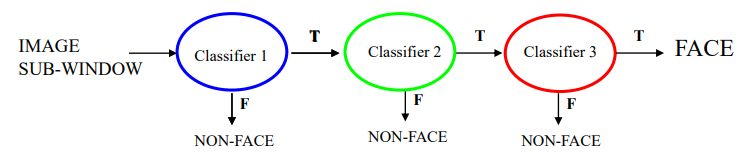
\includegraphics[height=2.25cm]{img/cascade_class.PNG}
    \caption{How multiple strong classifiers are chained to form a cascade one. The first cascale belongs to large scale (smallest image), the second to smaller scale, etc. Classifier 2 is activated by 1 and 3 by 2.}
    \label{fig:cascade_class}
\end{figure}
% ref https://www.cc.gatech.edu/~hays/compvision2017/lectures/23.pdf, https://www.cse.iitb.ac.in/~ajitvr/CS763_Spring2017/Adaboost_FaceDetection.pdf
We study how the length of the cascade improves its quality. Let $f_i$ be the False Positive Rate (FPR) of each classifier and $d_i$ is detection rate (True Positive Rate -- TPR\footnote{FPR and TPR are defined as follows. $P$ are the total positive and $N $ the total negative examples. $TPR = \frac{TP}{P}=\frac{TP}{TP+FN}$, $FPR = \frac{FP}{N} = \frac{FP}{FP+TN}$.}). Assuming the stages are independent, then the \textit{overall} false positive rate $F$ and the overall detection rate $D$ is
\begin{equation}
    F = \prod\limits_{i=1}^{K}f_i
\end{equation}
\begin{equation}
    D = \prod\limits_{i=1}^{K}d_i
\end{equation}
\marginnote{High FPR does not really affect the cascade's quality. However, TPR needs to be high.} Assume $K=10$. If every stage (assume they all preform roughly the same) has TPR $d_i=99\%$ and FPR $f_i = 40\%$, then the cascade  has $D = 0.99^{10}=90\%$ and $F = 0.4^{10} = 0.001\%$.

\subsubsection{Training the cascaded classifier}
Therefore having high FPR at each stage is not a bad thing but having low TPR is undesirable. Hence, training the whole cascade is summarised as follows.
% ref http://vision.cs.utexas.edu/378h-fall2015/slides/lecture20.pdf
\begin{enumerate}
    \item Set target detection and false positive rates for each stage.
    \item Keep adding features to the current stage until its target rates have been met.
    \begin{enumerate}
        \item Need  to lower AdaBoost threshold  to maximise detection (as opposed  to minimising total classification  error).
        \item Test  on a validation set.
    \end{enumerate}
    \item If the overall false positive rate is not low enough, then add another stage.
    \item Use false positives from current stage as the negative training  examples for the next stage.
\end{enumerate}
Training could, for instance, include $5\cdot 10^3$ positives, $350\cdot 10^6$ negatives, and could result in a real-time cascaded detector with $38$ stages and $6061$ features along all layers. The figure below how individual classifiers, each with its own Haar features, could look like.

\begin{figure}[H]
    % ref http://www.egr.unlv.edu/~b1morris/ecg782/slides/viola_jones_face_detection.pdf
    \centering
    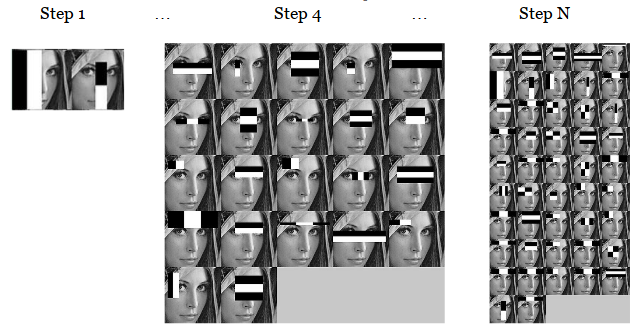
\includegraphics[height=4.5cm]{img/cascade_vis.png}
    \caption{The first weak classifier has in this case 2 simple features , outputting lots of FP. The rest have progressively more features.}
\end{figure}




\subsection{Face and object detection in OpenCV}

As mentioned before, the cascade Viola Jones classifier can work in real time thanks to the cascade of strong classifiers, which are applied sequentially. Although we could have thousands of features, they are not applied at the same time. The first classifier contains the fewest features, the second more etc. If at any stage the input image does not pass one of the classifiers, it's rejected. This saves huge amounts of computation time.

Object, not only face, detection in OpenCV is very straightforward. First, we initialise a \mintinline{python}{cv2.CascadeClassifier} object:
\begin{minted}{python}
cv2.CascadeClassifier(xml_file) -> cascade_detector
\end{minted}
\begin{itemize}
    \item \mintinline{python}{xml_file} is the path to an .xml file that contains training data, i.e. the Haar features and threshold of each classifier stage. It contains data in a special format. Some samples can be found in \href{https://github.com/opencv/opencv/tree/master/data/haarcascades}{OpenCV's repository}. Note that the \mintinline{latex}{.xml} files contain also features trained to detect face profiles, eyes, bodies, etc.
    \item \mintinline{python}{cascade_detector} is the object that will actually run the Viola-Jones algorithm. More on it next.
\end{itemize}
\begin{minted}{python}
cv2.CascadeClassifier.detectMultiScale(image[, scaleFactor[, minNeighbors[, flags[,
minSize[, maxSize]]]]]) -> objects
\end{minted}
% doc: https://docs.opencv.org/3.4/d1/de5/classcv_1_1CascadeClassifier.html#aaf8181cb63968136476ec4204ffca498
\begin{itemize}
    \item \mintinline{python}{image}: Greyscale image that contains objects to be detected.
    \item \mintinline{python}{scaleFactor}: Specifies how much the image size is reduced at each image scale. Default value is \mintinline{python}{1.2}.
    \item \mintinline{python}{minNeighbors}: Specifyies how many neighbors each candidate rectangle should have to retain it. Default value is \mintinline{python}{3}.
    \item \mintinline{python}{flags}: Parameter with the same meaning for an old cascade as in the function cv2.HaarDetectObjects. It is not used for a new cascade.
    \item \mintinline{python}{minSize}: A tuple. Minimum possible object size. Objects smaller than that are ignored.
    \item \mintinline{python}{maxSize}: A tuple. Maximum possible object size. Objects larger than that are ignored. If \mintinline{python}{maxSize == minSize} model is evaluated on single scale.
    \item \mintinline{python}{objects}: An array of rectangles. Each rectangle is, in turn, an array \mintinline{python}{x0, y0, width, height}.
\end{itemize}
If the input image has low constrast, OpenCV suggests histogram pre-processing before applying the face detector.

\mintinline{python}{scaleFactor} may need to be calibrated depending on how large the face to detect is relative to the image size. Recall that scale factor defines how much the image is downsampled from one pyramid level to another. For example, if the input image has resolution $1280\times 800$ and \mintinline{python}{scaleFactor = 1.2}, then the pyramid base level has size $1280\times 800$ and the next has $20\%$ of it, so $1168\times 730$ and so forth. Reducing the scale factor increases the chance of finding a face but also increases computation time and also false positives. 

Decreasing \mintinline{python}{minNeighbors} increases the number of detection rectangles that can overlap each other.

The code is listed in \ref{app:viola_jones_cv} and a result is shown below.
\begin{figure}[H]
    \centering
    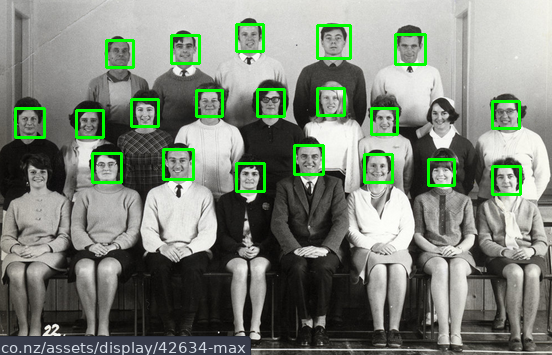
\includegraphics[height=4.5cm]{img/viola_jones_out.png}
    \caption{Applying Viola-Jones for \mintinline{python}{scalingFactor = 1.1} and \mintinline{python}{minNeighbors = 5}.}
\end{figure}



\subsection{How to train your own cascade classifier in OpenCV}


\marginnote{Requirement: OpenCV 3.x}OpenCV 3.x allows you to train your own cascade classifier. Cascade training has been dropped in version 4.x. The way it works is 
\begin{enumerate}
    \item Prepare the directory structure.
    \item Grab some positive and negative images and store them in the directory.
    \item (Optional) Augment the positive datasets, e.g. randomly rotate, flip, or add noise to each positive image.
    \item Generate the metadata, such information files regarding where the images are and the object location in the positive images.
    \item Do the training. This is will eventually generate an \mintinline{latex}{.xml} file that is usable for the target object detection.
\end{enumerate}
Before deciding on an object to train the classifier for, it it worth asking yourself whether it's susceptible to Haar feature detection. The object to detect must consistently have certain features at certain positions relative to each other, so that when Haar rectangles cover them, they are able to produce high differences. For example, for a clenched fist detector these features could be the dark ridges between the fingers, the thumb, the nails at the end etc. For an orange detector it would be hard to come up with such features as the shape is generic and other than the pores, not many indicators exist for the classifier to tell it apart e.g. from a ball.
There are many similar ways to do the training but below is the one that works for me.



\subsubsection{Prepare the directory structure}

On github there is already an empty repository that's fit for cascade training. Clone it
\begin{lstlisting}[style=terminal]
git clone https://github.com/0xLeo/opencv-haar-classifier-training.git
cd opencv-haar-classifier-training/
\end{lstlisting}
Remove all the \mintinline{latex}{.gitkeep} files so that they're not accidentally included as training images.
\begin{lstlisting}[style=terminal]
find . -type f -name .gitkeep -exec rm -f {} \;
\end{lstlisting}
After cloning, the directory structure should look as follows:
\begin{verbatim}
.
+-- bin
|   +-- createsamples.pl
+-- classifier
+-- LICENSE
+-- negative_images
+-- positive_images
+-- README.md
+-- samples
+-- tools
|   +-- <files>
+-- trained_classifiers
    +-- <files>
\end{verbatim}



\subsubsection{Collect positive and negative training images}

Remember two things when downloading training images.
\begin{enumerate}
    \item The positive images should contain only the object of interest and as little margin around it as possible.
    \begin{enumerate}
        \item The reason we want the background margin around the OOI to be as narrow as possible is to facilitate object annotation in the next sections.
        \item Cropping may be required to get a good representation of the OOI. After cropping, remember that all positive images (OOI) must have roughly the same $\textup{width}:\textup{height}$ ratio. The reason for this will be clear in the augmentation section.
    \end{enumerate}
    \item The negative images can contain anything but the object of interest (OOI). Ideally, they contain objects or scenes that can be found in the background.
\end{enumerate}
. To quickly crop the object, a tool such as  \href{https://www.batchcrop.com}{batchcrop} is recommended. Unfortunately, this only works on Windows. 

A way of collecting positive images is by downloading pre-compiled datasets and extracting their RGB images and cropping the OOI. Alternatively, videos can be converted to images. A few thousand positive and a few thousand negatives should be fine. Once they have been collected and cropped and follow guidelines (1) and (2), dataset augmentation can begin. When done collecting the images and cropping the positives, copy them to \texttt{positive\_images} and \texttt{negative\_images}. 

After copying them, it it recommended to convert the negative images to grayscale. This is done by configuring and runing the augmentation tool found in \texttt{tools} directory. Then edit the tool's config, found in \texttt{augment\_config.yaml} so that only grayscale conversion is enabled, run the tool from \texttt{main.py}. If there are any non-grayscale images (they do not contain \texttt{gray} in their name) left in the \texttt{negative\_images}, delete them manually.
\begin{lstlisting}[style=terminal]
edit augment_config.yaml
config:
    directory: ../negative_images/ 
    grayscale: yes
    equalise: no
    rotate:
        flag: no
        how_many: 6
        min_angle: -25
        max_angle: 25
    flip:
        flag: no
    noise:
        flag: no 
        var: 0.6
    resize:
        flag: no
        width: 128
        height: 128
./main.py
\end{lstlisting}

\textbf{Tip}:  \texttt{christopher5106}   \footnote{\faExternalLinkSquare
 \; \url{http://christopher5106.github.io/computer/vision/2015/10/19/create-an-object-detector.html}} on github recommends that ``each (negative) image should be (but not necessarily) larger than a training window size, because these images are used to subsample negative image to the training size''. The reason he recommends it is that so that only the exact negative image can be used during training, and not random parts of it. I tried it, but it \textit{didn't improve my results} compared to no resizing -- it only introduced more FPs.  
 
\marginnote{Negative images need to be converted to grayscale.}\textbf{Tip:} I found that the more positives used for training, the more FP the classifier is likely to detect and the more negatives, the more FN the it's likely to detect. So a workflow is to test the trained classifier, check whether is detects too many FP and FN and balance the dataset accordingly. You can begin with a ratio  \texttt{pos:neg = 3:2}  and check the trained classifier's results.



\subsubsection{Augment the positive dataset}

Image data augmentation is a technique that can be used to artificially expand the size of a training dataset by creating modified versions of the postive images in the dataset. It therefore allows the model to generalise its results. Augmentation can be done by the \texttt{opencv\_createsamples} command but that didn't work for me so I used my own tool.

\marginnote{Run the augmentation tool on positive images.}If you have collected e.g. a few hundred positive images, augmentation first performs pre-processing (conversion to grayscale followed by histogram equalisation) and create a flipped copy of each one, randomly rotate it a number of times and add noise to the result if necessary, therefore generate new positive images based on the existing ones. The class to perform augmentation is found in \texttt{tools/augment.py} and its config in \texttt{tools/augment\_config.yaml}. You need to modify the latter file to meet your needs. The file contents were also listed in the previous section. When done, augmentation of positive samples can begin by running.
\begin{lstlisting}[style=terminal]
chmod +x main.py
./main.py
\end{lstlisting}
When done, the \texttt{positive\_images} folder should only contain grayscale images of the same size. They will contain either \texttt{resized} or \texttt{augm} in their filename. If anything else exists in the folder, remove it manually.



\subsubsection{Generate the metadata and the vector file}

OpenCV needs a file to list positives, one to list negatives and one to list obj locations in positives images.
\begin{lstlisting}[style=terminal,language=bash]
cd <project_root>
find ./positive_images/ -iname *.png > positives.txt
find ./negative_images/ -iname *.png > negatives.txt
\end{lstlisting}
Positive images should only contain \texttt{.png} images. If you haven't converted the negtive images to grayscale by the tool and they still contain \texttt{.jpg}, \texttt{.tiff} etc, you need to append them like so:
\begin{lstlisting}[style=terminal]
find ./negative_images/ -iname *.jpg >> negatives.txt
\end{lstlisting}
\textbf{Tip:} None of the images, either positive or negative, must contain spaces in its file name. This is guaranteed for positive images as they should have been generated by the augmentation tool, but if negatives contain spaces remove them manually.

Now generate the file that contains the object positions as rectangles (info file). Since cropping is as tight as possible, we assume that the OOI takes the whole image. Info file is based on \mintinline{latex}{positives.txt} so in the project root, copy the latter:
\begin{lstlisting}[style=terminal]
cp positives.txt info.dat
\end{lstlisting}
In the end, we want each line of \texttt{info.dat} to look as follows:
\begin{verbatim}
<path_from_root_to_positive_image> <number_of_objects> <x0> <y0> <x1> <y1>
\end{verbatim}
The starting position of the rectangle around the OOI is $(0,0)$ and the end is $(image\_width, image\_height)$. For example, if all images have been resized to $(128, 128)$, objects have been cropped correctly and each one contains only one object, then if you open the info file, each line of \mintinline{latex}{info.dat} should look like:
\begin{lstlisting}[style=terminal]
edit info.dat
./positive_images/resized_00212_rot_03.png 1 0 0 128 128
\end{lstlisting}
Once annotating is done, generate the \mintinline{latex}{.vec} file, which encodes all positive images together in a vector given the \mintinline{latex}{info.dat} file. However, the vector file should further resize the positives to the training size, otherwise training will be slow. In this case $128\times128$ is too large for training, so shrinking the positives is necessary. For this, we need the \mintinline{latex}{opencv_createsamples} program, which is part of OpenCV 3.x. The command to create a vector file (\mintinline{latex}{sampels.vec}) containing all positive images downsampled to $36\times 36$ is:
\begin{lstlisting}[style=terminal]
NPOS=`cat positives.txt | wc -l`
opencv_createsamples -info info.dat -vec samples.vec -h 36 -w 36 -num $NPOS
\end{lstlisting}
To make sure the vector is created correctly, view the generated images with the following command and press escape to close the window:
\begin{lstlisting}[style=terminal]
opencv_createsamples -vec samples.vec  
\end{lstlisting}




\subsubsection{Do the training}

Before the training begins, make sure the directory where the cascade classifier  will be writing (specified by the \texttt{-data} options below) the training weights for each stage and the final classifier is empty:
\begin{lstlisting}[style=terminal]
mkdir -p classifier
rm classifier/*
\end{lstlisting}
Use the following command for training. Adjust the parameters to your needs.
\begin{lstlisting}[style=terminal]
opencv_traincascade -data classifier -vec samples.vec -bg negatives.txt
-acceptanceRatioBreakValue 0.00001 -minHitRate 0.995 -maxFalseAlarmRate 0.35 
-numPos 2850 -numNeg 1678 -w 36 -h 36 -mode ALL -precalcValBufSize 1024
-precalcIdxBufSize 1024 -featureType LBP
\end{lstlisting}



\textbf{Tip:} If your minHitRate is too high, you may get the following error:
\begin{verbatim}
imagestorage.cpp:159: error: (-5) Can not get new positive sample.
The most possible reason is insufficient count of samples in given vec-file. 
\end{verbatim}
This means that the classifier does not have enough information to reach the required \texttt{minHitRate} or \texttt{maxFalseAlarmRate}. To continue, either decrease \texttt{minHitRate} and increase \texttt{maxFalseAlarmRate} and continue the training or get more positive samples, augment them, annotate them, and restart the training.
The parameters that need to be explained are the following. For more, see the help menu of the command.
\begin{itemize}
    \item \mintinline{latex}{data}: The output file where the training weights and the final .xml, called cascade.xml will be written.
    \item \mintinline{latex}{numStages}: Number of stages of cascade classifier.
    \item \mintinline{latex}{minHitRate}: Minimum TP rate of each stage of the classifier. It needs to be high as, if it's e.g. $0.99$, for 16 stages the final TP rate would be $0.99^{16} \approx 0.851$. 
    \item \mintinline{latex}{maxFalseAlarmRate}: Maximum FP rate of each stage. If for one stage FPR is $0.35$, then for 16 stages the final is $0.35^{16} \approx 0$.
    \item \mintinline{latex}{numPos}: Number of positive images used for learning at each stage.
    \item \mintinline{latex}{numNeg}: Likewise, for negative images.
    \item \mintinline{latex}{w, h}: The width and height of images stored in the .vec file.
    \item \mintinline{latex}{featureType}: can be either \mintinline{latex}{LPB} or \mintinline{latex}{HAAR}. LPB stands for Local Binary Patterns and it's a similar type of  features to Haar as it uses Haar features. LPB uses integer arithmetic and HAAR floating point, therefore LPB is several times faster but slightly less accurate.
\end{itemize}

\marginnote{A good rule of thumb when to stop the training is when \texttt{1e-4 <= acceptance}
\texttt{RatioBreak}
\texttt{Value <= 1e-5} }\textbf{Tip}: According to the OpenCV documentation, if \texttt{acceptanceRatio}
\texttt{BreakValue} has been set for training, A good guideline is to train not further than 1e-4, to ensure the model does not overtrain on your training data. For me good, non-overfitting results we

While the training is ongoing, it will display an output similar to the following.
\begin{verbatim}
===== TRAINING 0-stage =====
<BEGIN
POS count : consumed   2300 : 2300
NEG count : acceptanceRatio    430 : 1
Precalculation time: 13
+----+---------+---------+
|  N |    HR   |    FA   |
+----+---------+---------+
|   1|        1|        1|
+----+---------+---------+
|   2|        1|        1|
+----+---------+---------+
|   3|        1|        1|
+----+---------+---------+
|   4|        1| 0.909302|
+----+---------+---------+
|   5|        1|      0.9|
+----+---------+---------+
|   6|        1| 0.695349|
+----+---------+---------+
|   7|        1| 0.723256|
+----+---------+---------+
|   8|        1| 0.634884|
+----+---------+---------+
|   9|        1| 0.327907|
+----+---------+---------+
END>
Training until now has taken 0 days 0 hours 0 minutes 24 seconds.
\end{verbatim}
When it's done, it will generate the trained classifier at \mintinline{latex}{classifier/cascade.xml}. Then, for example the program at \ref{app:viola_jones_cv} can be used to test it. If you want to train a new classifier, delete the contents of the \texttt{classifier} directory:
\begin{lstlisting}[style=terminal]
rm classifier/*
\end{lstlisting}
In the next section there are some real-world results of my Haar hand detector.


\subsection{A trained hand classifier}

A classifier that detects the following hand gestures 
\begin{enumerate}
    \item clenched fingers/ fist
    \item index finger raised
    \item index and middle finger raised
\end{enumerate}
, best at indoor light conditions, has been stored as \texttt{.xml} file at \footnote{\faExternalLinkSquare \; \url{https://github.com/0xLeo/opencv-haar-classifier-training/blob/master/trained_classifiers/hand_44x44_19_stages_lbp.xml}}. To try it, or another trained classifier, on a webcam, use the code at \ref{app:real_time_detector}. Below are some of its outputs.


\begin{multicols}{3}

\begin{figure}[H]
    \centering
    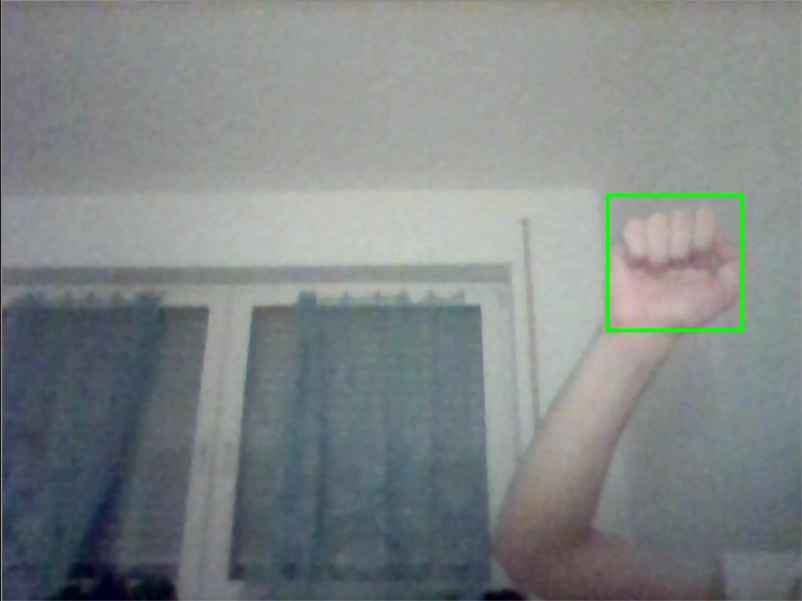
\includegraphics[width=0.3\textwidth]{img/hand_detector_out1.png}
    \caption{Fist with light background. }
\end{figure}
\columnbreak

\begin{figure}[H]
    \centering
    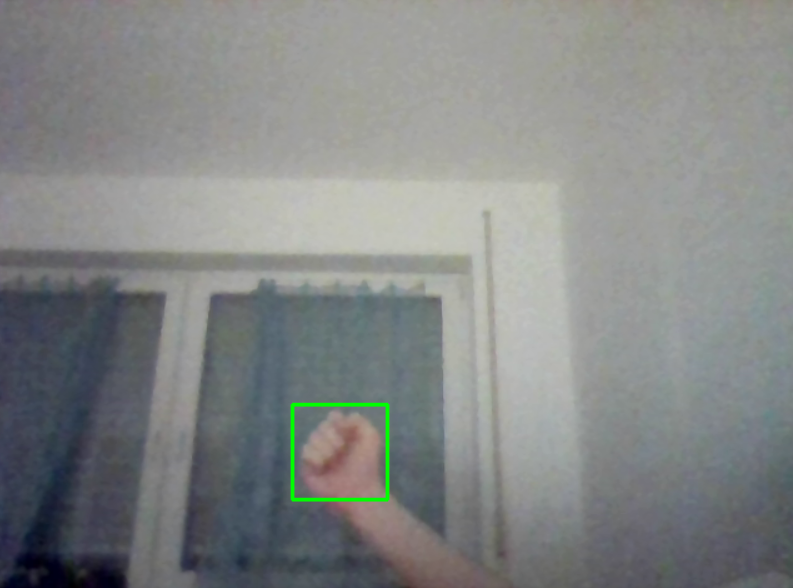
\includegraphics[width=0.3\textwidth]{img/hand_detector_out2.png}
    \caption{Fist with dark background.}
\end{figure}
\columnbreak

\begin{figure}[H]
    \centering
    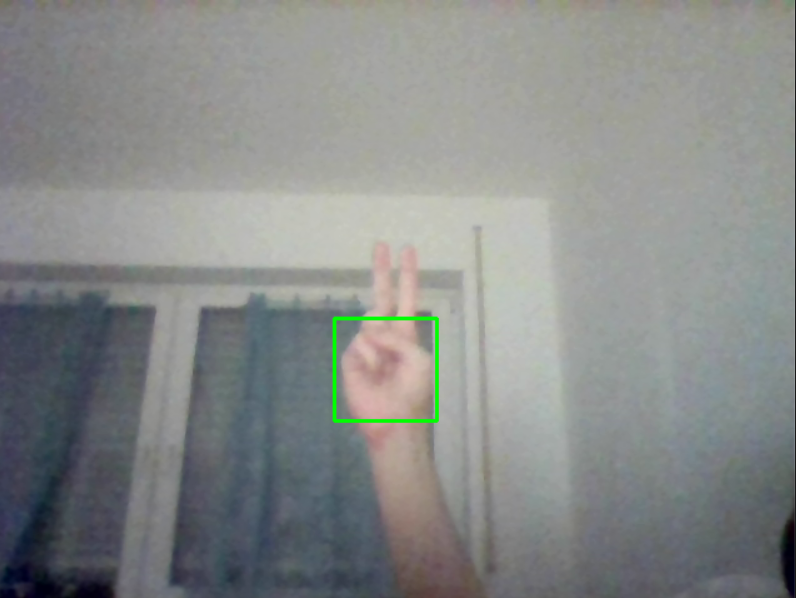
\includegraphics[width=0.3\textwidth]{img/hand_detector_out3.png}
    \caption{Victory sign.}
\end{figure}
\end{multicols}



%=-=-=-=-=-=-=-=-=-=-=-=-=-=-=-=-=-=-=-=-=-=-=-=-=-=-=-=-=-=-=-=-=-=-=-=-=-=-=-=-
% Appendices
%=-=-=-=-=-=-=-=-=-=-=-=-=-=-=-=-=-=-=-=-=-=-=-=-=-=-=-=-=-=-=-=-=-=-=-=-=-=-=-=-
\newpage
\appendix

\section{Appendices}

% ------------------------ New appendix ------------------------ %
\newpage
\subsection{Viola Jones in OpenCV}
\label{app:viola_jones_cv}

\lstinputlisting[language=python,caption={Python implementation (\detokenize{src/viola_jones_cv.py)}.}, label=src:mylabel]{src/viola_jones_cv.py}


% ------------------------ New appendix ------------------------ %
\newpage
\subsection{Real-time cascade detector in OpenCV}
\label{app:real_time_detector}

\lstinputlisting[language=python,caption={Detecting an object in real time given an .xml file (\detokenize{src/viola_real_time.py)}.}]{src/viola_real_time.py}


%=-=-=-=-=-=-=-=-=-=-=-=-=-=-=-=-=-=-=-=-=-=-=-=-=-=-=-=-=-=-=-=-=-=-=-=-=-=-=-=-
% References
%=-=-=-=-=-=-=-=-=-=-=-=-=-=-=-=-=-=-=-=-=-=-=-=-=-=-=-=-=-=-=-=-=-=-=-=-=-=-=-=-
\newpage
\printbibliography


\end{document}